% Back Cover — "Spectrum Flow" companion to cover-5
\documentclass[tikz,border=0mm]{standalone}
\usepackage{tikz}
\usetikzlibrary{calc}
\usepackage{xcolor}
\usepackage[T1]{fontenc}

\definecolor{deeppurple}{RGB}{22,6,50}
\definecolor{paneldark}{RGB}{15,4,36}
\definecolor{tealdeep}{RGB}{0,78,90}
\definecolor{tealbright}{RGB}{65,215,195}
\definecolor{tealaccent}{RGB}{110,235,218}
\definecolor{lavender}{RGB}{172,132,215}
\definecolor{lavlight}{RGB}{205,178,238}
\definecolor{peach}{RGB}{238,148,85}
\definecolor{peachlight}{RGB}{252,190,140}
\definecolor{whitesoft}{RGB}{244,241,255}
\definecolor{whitedim}{RGB}{170,165,195}
\definecolor{panelmid}{RGB}{12,35,48}

\begin{document}
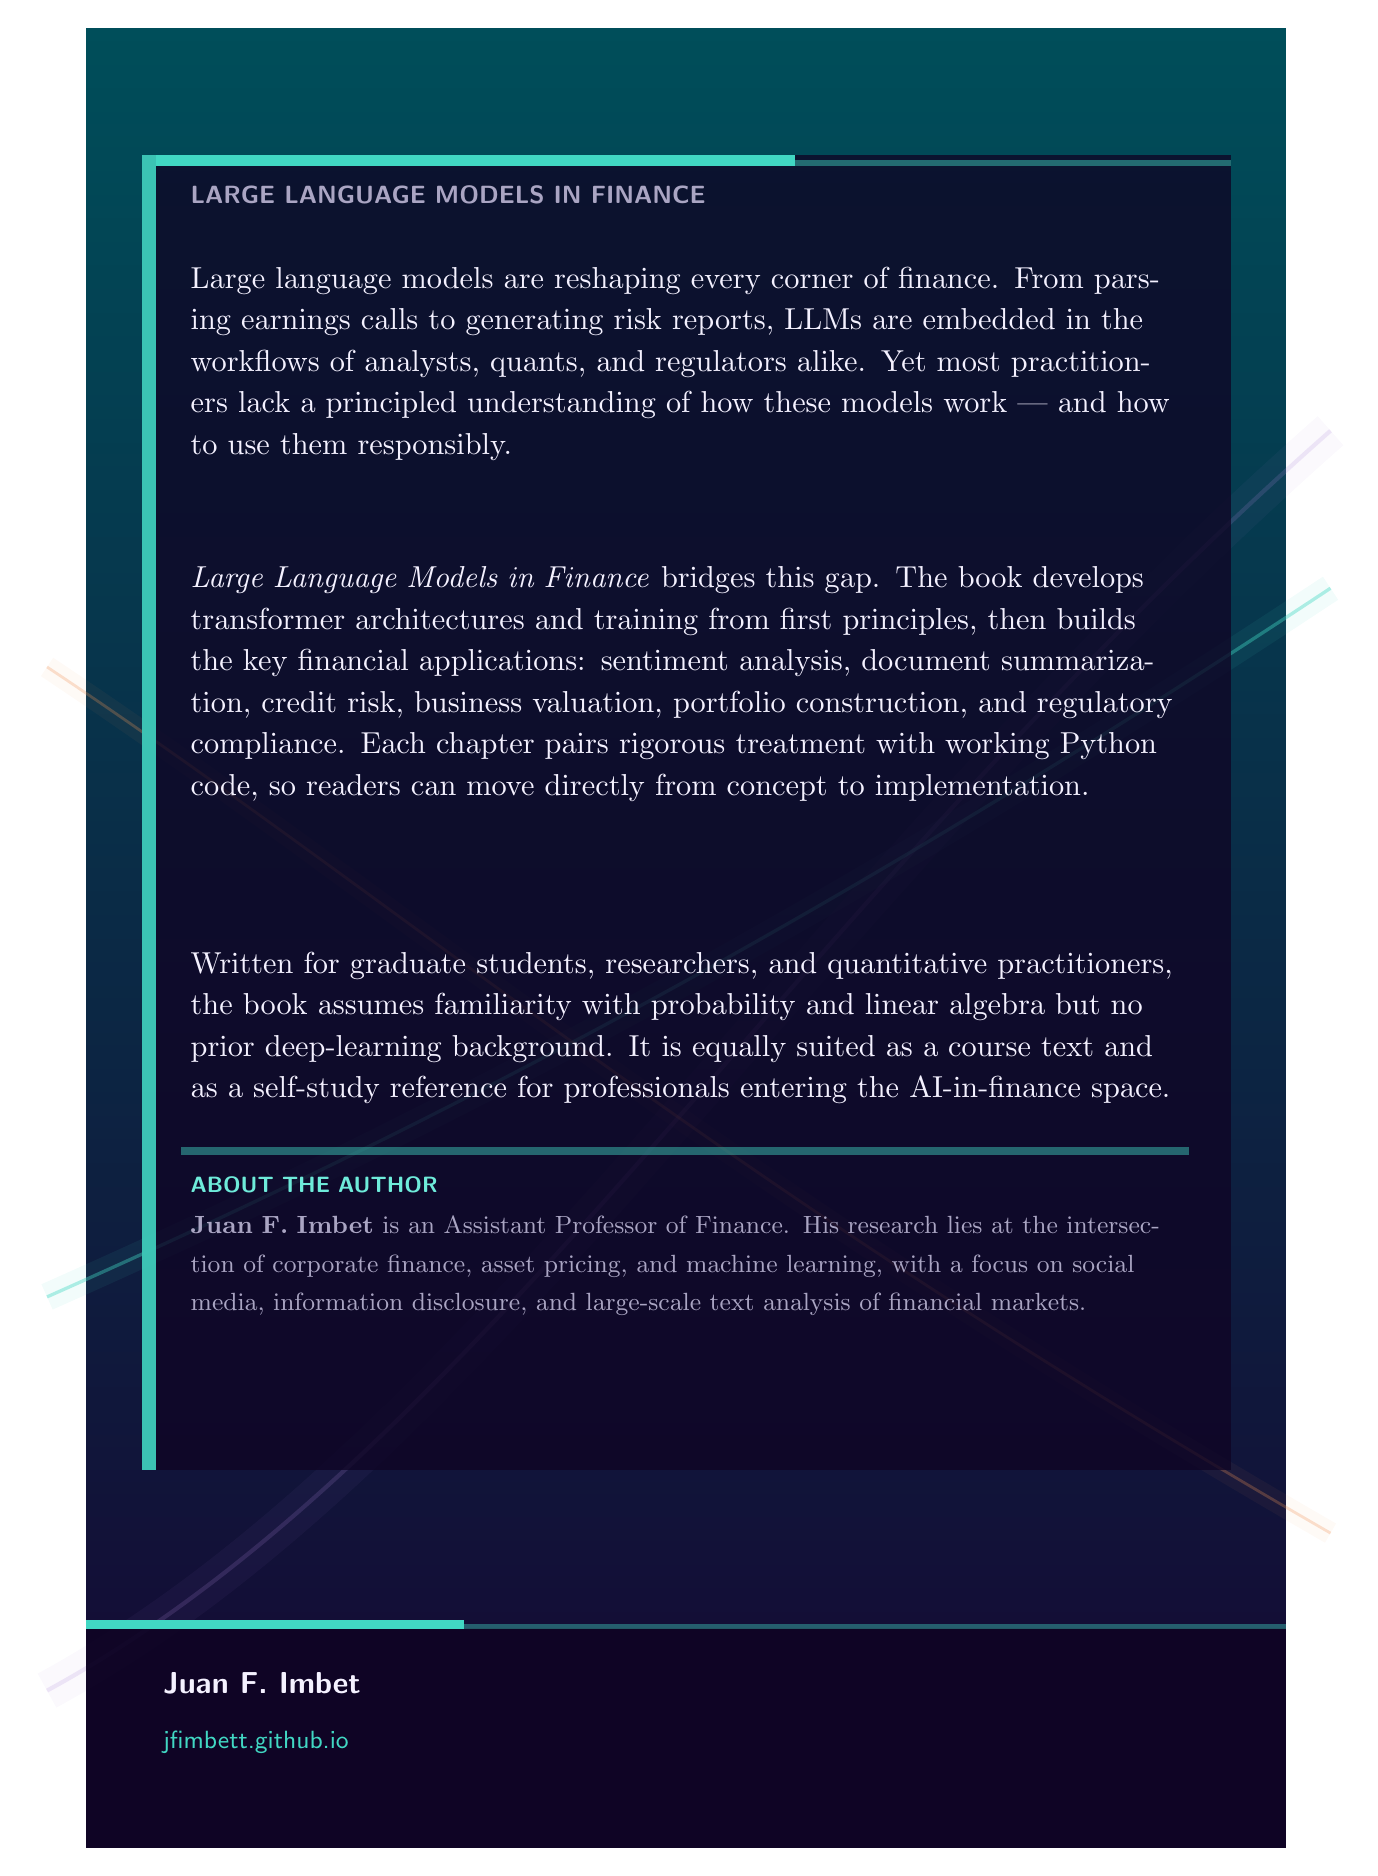
\begin{tikzpicture}

  % ── GRADIENT BACKGROUND (same as front) ────────────────────────────────────
  \foreach \y in {0,0.15,...,23.0}{
    \pgfmathsetmacro{\t}{\y/22.86}
    \pgfmathsetmacro{\r}{int(22 + (0-22)*\t)}
    \pgfmathsetmacro{\g}{int(6  + (78-6)*\t)}
    \pgfmathsetmacro{\b}{int(50 + (90-50)*\t)}
    \definecolor{bkg}{RGB}{\r,\g,\b}
    \fill[bkg] (0,\y) rectangle (15.24,\y+0.17);
  }

  % ── BACKGROUND STREAMS (subtle — behind text) ──────────────────────────────
  \draw[lavender,line width=14pt,opacity=0.05]
    (-0.5,2.0) .. controls (5,5) and (9,12) .. (15.8,18.0);
  \draw[lavender,line width=1.5pt,opacity=0.18]
    (-0.5,2.0) .. controls (5,5) and (9,12) .. (15.8,18.0);

  \draw[tealbright,line width=10pt,opacity=0.07]
    (-0.5,7.0) .. controls (4,9) and (9,11.5) .. (15.8,16.0);
  \draw[tealbright,line width=1.2pt,opacity=0.40]
    (-0.5,7.0) .. controls (4,9) and (9,11.5) .. (15.8,16.0);

  \draw[peach,line width=8pt,opacity=0.05]
    (-0.5,15) .. controls (4,12) and (8,8.5) .. (15.8,4.0);
  \draw[peach,line width=1.0pt,opacity=0.28]
    (-0.5,15) .. controls (4,12) and (8,8.5) .. (15.8,4.0);

  % ── FROSTED TEXT PANEL ─────────────────────────────────────────────────────
  \fill[paneldark,opacity=0.78] (0.7,4.8) rectangle (14.54,21.5);

  % teal left-edge accent
  \fill[tealbright,opacity=0.90] (0.7,4.8) rectangle (0.88,21.5);

  % top teal rule inside panel
  \fill[tealbright,opacity=1.0]  (0.88,21.36) rectangle (9.0,21.50);
  \fill[tealbright,opacity=0.45] (9.0,21.36)  rectangle (14.54,21.44);

  % ── TITLE LINE (small, top of panel) ───────────────────────────────────────
  \node[anchor=west,text=whitedim,font=\fontsize{9}{11}\selectfont\sffamily\bfseries]
    at (1.2,21.0) {LARGE LANGUAGE MODELS IN FINANCE};

  % ── BLURB ──────────────────────────────────────────────────────────────────
  \node[anchor=north west,text=whitesoft,
        font=\fontsize{10.5}{15}\selectfont\rmfamily,
        text width=12.5cm, align=left]
    at (1.2,20.2) {%
Large language models are reshaping every corner of finance. From parsing earnings
calls to generating risk reports, LLMs are embedded in the workflows of analysts,
quants, and regulators alike. Yet most practitioners lack a principled understanding
of how these models work — and how to use them responsibly.
    };

  \node[anchor=north west,text=whitesoft,
        font=\fontsize{10.5}{15}\selectfont\rmfamily,
        text width=12.5cm, align=left]
    at (1.2,16.4) {%
\textit{Large Language Models in Finance} bridges this gap. The book develops
transformer architectures and training from first principles, then builds the key
financial applications: sentiment analysis, document summarization, credit risk,
business valuation, portfolio construction, and regulatory compliance. Each chapter
pairs rigorous treatment with working Python code, so readers can move directly
from concept to implementation.
    };

  \node[anchor=north west,text=whitesoft,
        font=\fontsize{10.5}{15}\selectfont\rmfamily,
        text width=12.5cm, align=left]
    at (1.2,11.5) {%
Written for graduate students, researchers, and quantitative practitioners, the
book assumes familiarity with probability and linear algebra but no prior
deep-learning background. It is equally suited as a course text and as a
self-study reference for professionals entering the AI-in-finance space.
    };

  % ── DIVIDER ────────────────────────────────────────────────────────────────
  \fill[tealbright,opacity=0.45] (1.2,8.8) rectangle (14.0,8.90);

  % ── ABOUT THE AUTHOR (mini) ─────────────────────────────────────────────────
  \node[anchor=north west,text=tealaccent,
        font=\fontsize{8}{9}\selectfont\sffamily\bfseries]
    at (1.2,8.65) {ABOUT THE AUTHOR};

  \node[anchor=north west,text=whitedim,
        font=\fontsize{9.5}{14}\selectfont\rmfamily,
        text width=12.5cm, align=left]
    at (1.2,8.15) {%
\textbf{Juan F.\ Imbet} is an Assistant Professor of Finance. His research lies
at the intersection of corporate finance, asset pricing, and machine learning,
with a focus on social media, information disclosure, and large-scale text
analysis of financial markets.
    };

  % ── BOTTOM AUTHOR / WEBSITE ────────────────────────────────────────────────
  \fill[paneldark,opacity=0.90] (0,0) rectangle (15.24,2.8);
  \fill[tealbright,opacity=1.0] (0,2.78) rectangle (4.8,2.90);
  \fill[tealbright,opacity=0.40] (4.8,2.78) rectangle (15.24,2.84);

  \node[anchor=west,text=whitesoft,
        font=\fontsize{11}{13}\selectfont\sffamily\bfseries]
    at (0.85,2.1) {Juan F.\ Imbet};
  \node[anchor=west,text=tealbright,
        font=\fontsize{9}{11}\selectfont\sffamily]
    at (0.85,1.35) {jfimbett.github.io};

\end{tikzpicture}
\end{document}
